\section{Data and Physical Constraints}

The data are raw temperature matrices rather than pseudo-color video. The main
TXT session contains 255 frames from a raster-like step-and-shoot acquisition.
All session detection and frame ordering use acquisition order, not filename
lexicographic order, because filename sorting creates false temperature
segments.

The relevant physical constants are fixed before SR experiments:

\begin{itemize}
\item detector output: 640 by 480 pixels;
\item TXT sampling pitch: 10 um per pixel;
\item calibrated spatial resolution: about 20 um;
\item LWIR band: 8--14 um;
\item noise floor: about 0.0724 C;
\item stage-to-pixel rotation prior: 47.6 degrees.
\end{itemize}

\begin{figure}[t]
\centering
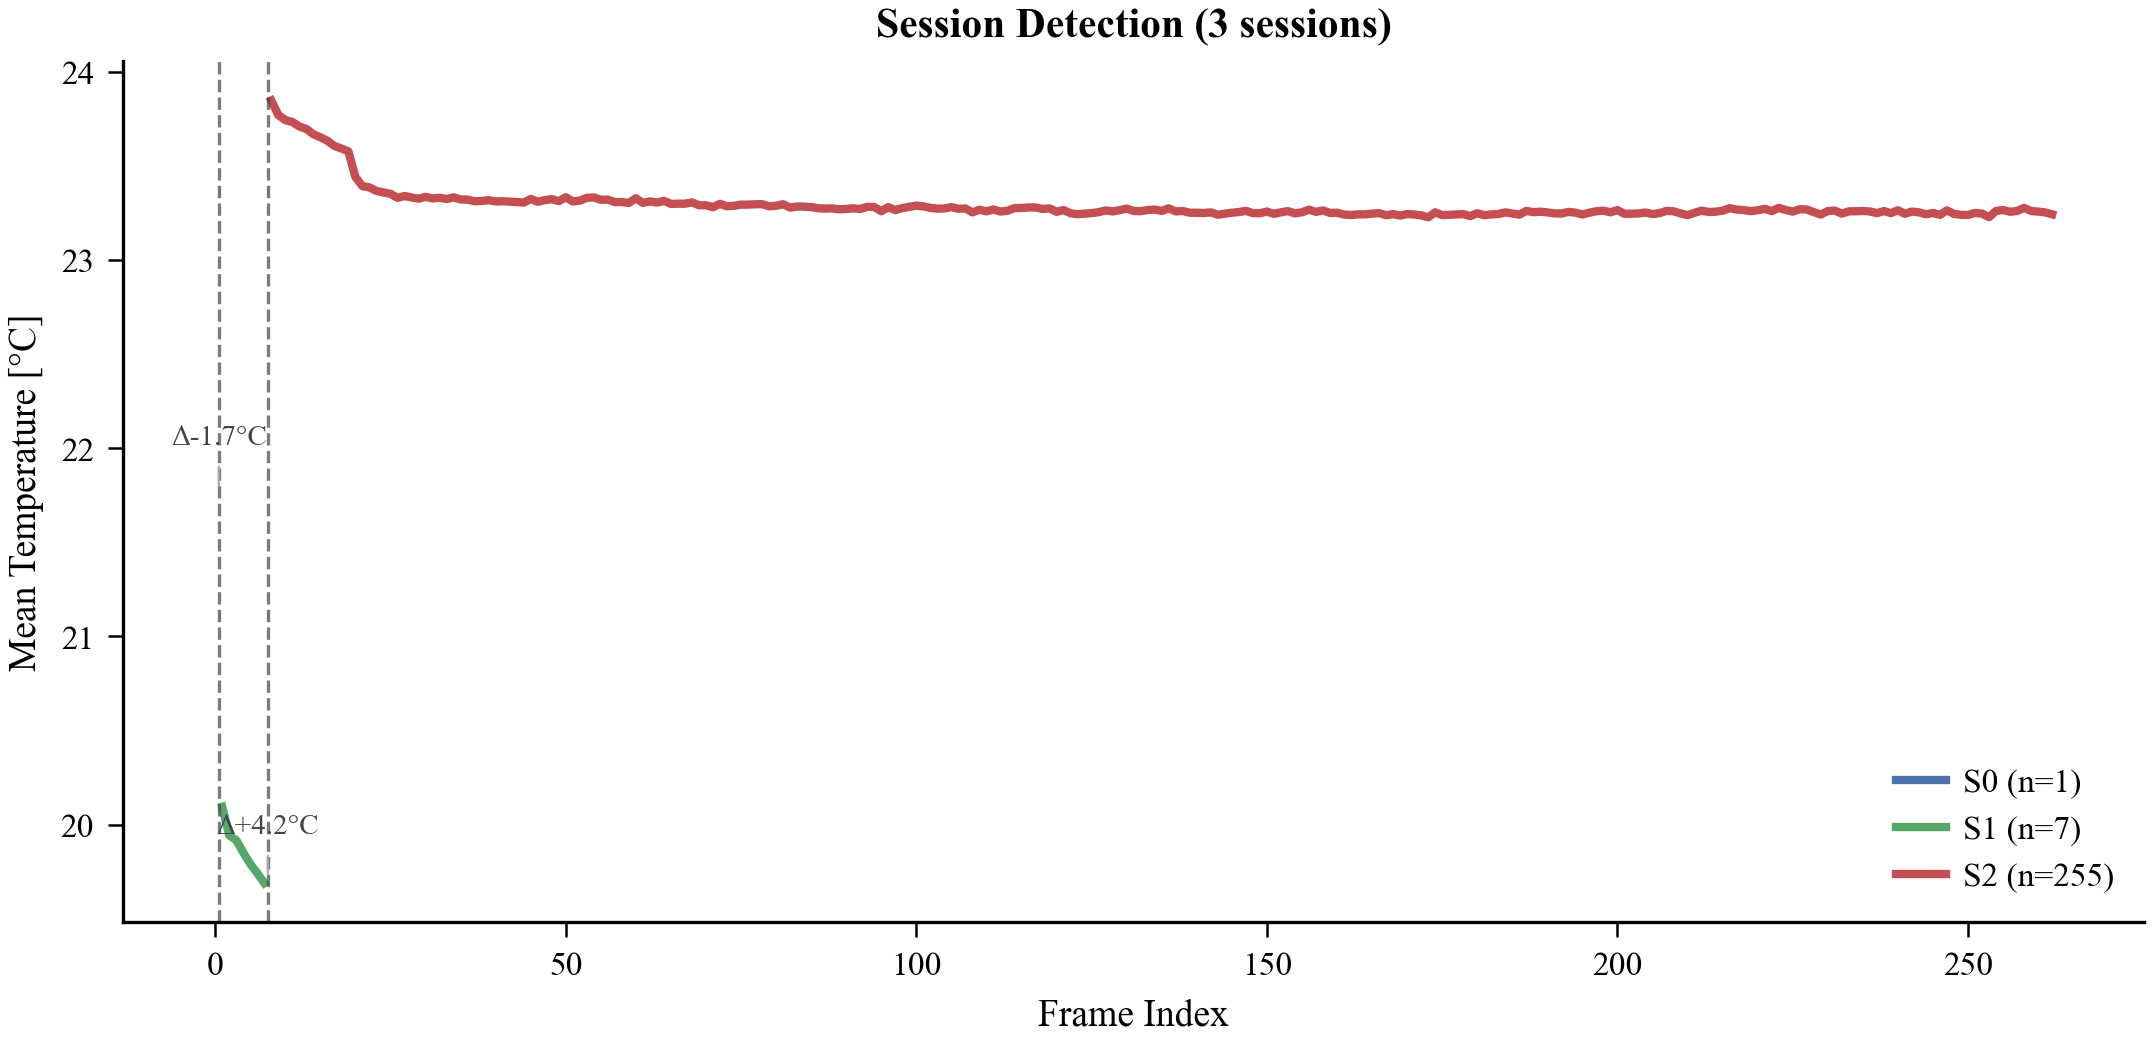
\includegraphics[width=\linewidth]{../figures/ep01_session_detection.png}
\caption{Main-session selection is based on acquisition order and temperature
state. Cross-session mixing is excluded from the SR inputs.}
\label{fig:session}
\end{figure}

The optical and thermal limits matter for interpretation. A 2x output grid
provides a denser reconstruction lattice, not a direct claim that the system now
resolves 5 um structure. The POC is evaluated as contour visibility and
stability, not absolute-temperature metrology.

